\documentclass{article}
\usepackage{amsfonts, amsmath, amssymb, amsthm} % Math notations imported
\usepackage{enumitem}
\usepackage{graphicx}
\usepackage[margin=1in]{geometry}
\usepackage{setspace}
\usepackage{tabularx}
\usepackage{indentfirst}
\graphicspath{{./images/}} % Path to images

% \begin{figure}[htb!]
%      \centering
%      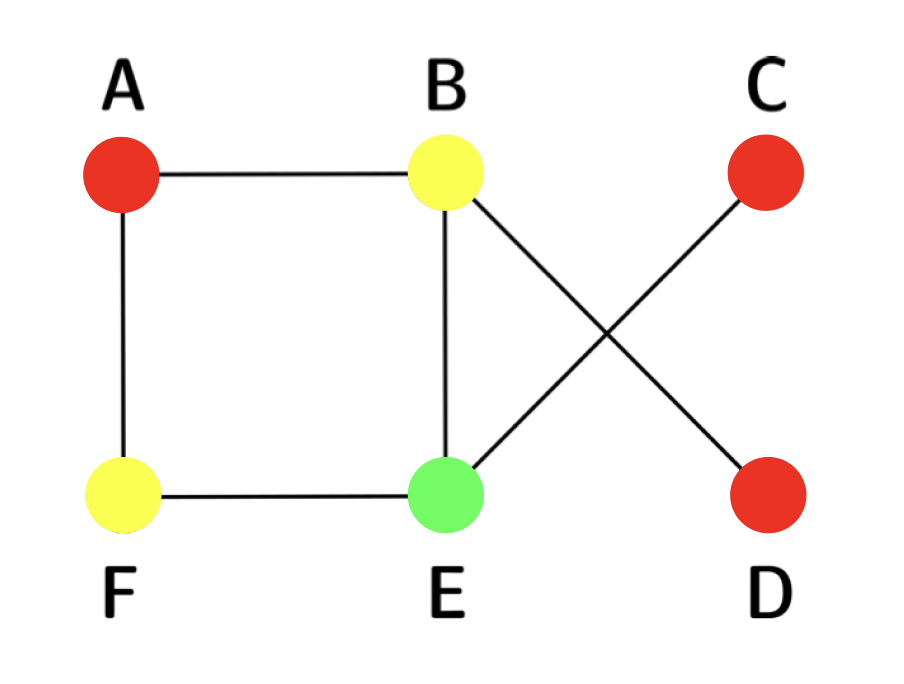
\includegraphics[scale=0.5]{coloring.png}
%      \caption{Coloring of the graph.}
% \end{figure}

\newtheorem{thm}{Theorem}
\newtheorem{proposition}[thm]{Proposition}
\newtheorem{cor}[thm]{Corollary}

% title information
\title{Math 110 HW1}
\author{Neo Lee}
\date{09/02/2023}

\setstretch{1.15}
% main content
\begin{document} 

% placing title information; comment out if using fancyhdr
\maketitle 

\section*{Problem 1}
Determine which complex numbers $x$ satisfy the equation $x^3 + x^2 + x + 1 = 0$.
\begin{proof}[Solution]
    \begin{align*}
        x^3 + x^2 + x + 1 & = 0 \\
        (x+1)(x^2+1) & = 0.
    \end{align*}
    
    For $x + 1 = 0$, $\underline{x = 1 + 0i}$.

    For $x^2 + 1 = 0, x^2 = -1 \Rightarrow \underline{x = 0 + i}$ or $\underline{x = 0 - i}$. 
\end{proof}

\section*{Problem 2}
Does there exist a complex number $\lambda$ such that $\lambda (2-3i, 5+4i, -6+7i) = 
(2+i, 3-i, 4)$?
\begin{proof}[Solution]
    We will evaluate the coordinates separately.
    
    Consider
    \begin{align*}
        \lambda (2-3i) & = 2+i \\
        \lambda & = \frac{2+i}{2-3i} \\
        \lambda & = \frac{(2+i)(2+3i)}{13} \\
        \lambda & = \frac{1 + 8i}{13}.
    \end{align*}

    Now consider
    \begin{align*}
        \lambda (5+4i) & = \frac{(1+8i)(5+4i)}{13} \\
        & = \frac{-27 + 44i}{13} \\
        & \neq 3 - i.
    \end{align*}

    We can see there does not exist $\lambda$ that satisfies both $x$ and $y$ coordinates. Hence, 
    there does not exist a complex solution to the equation.
    
\end{proof}

\section*{Problem 3}
Suppose that $\{0, 1, x\}$ is a field with exactly three elements. What do the addition and 
multiplication tables have to be in that case? Based on the addition and multiplication tables you 
get, check this is indeed a field. What is the 'natural' way to think of this field (and of x)?
\begin{proof}[Solution] \indent 
    \\
    \begin{align*}
        \begin{tabularx}{0.4\textwidth} { 
            | >{\centering\arraybackslash}X 
            | >{\centering\arraybackslash}X 
            | >{\centering\arraybackslash}X 
            | >{\centering\arraybackslash}X | }
           \hline
           + & 0 & 1 & $x$ \\
           \hline
           0  & 0  & 1 & $x$  \\
           \hline
           1  & 1  & $x$  & 0 \\
           \hline
           $x$  & $x$  & 0 & 1 \\
          \hline
        \end{tabularx} \qquad
        \begin{tabularx}{0.4\textwidth} { 
            | >{\centering\arraybackslash}X 
            | >{\centering\arraybackslash}X 
            | >{\centering\arraybackslash}X 
            | >{\centering\arraybackslash}X | }
           \hline
           $\times$ & 0 & 1 & $x$ \\
           \hline
           0  & 0  & 0 & 0  \\
           \hline
           1  & 0  & 1 & $x$ \\
           \hline
           $x$  & 0  & $x$ & 1 \\
          \hline
        \end{tabularx}
    \end{align*}

    Based on the tables, we can see that indeed the field is closed under addition and 
    multiplication. The field has additive and multiplicative identities, and every element has an
    additive and multiplicative inverse. Also, addition and multiplication are commutative since 
    the tables are symmetric about the main diagonal. We can also check that addition and 
    multiplication are indeed associative by simply listing all the possible cases. We can check 
    that distributive law holds in the same manner, but we will omit the proof here. Hence, we can 
    conclude that $\{0, 1, x\}$ is a field.

    The natural way to think of the field is to define addition as addition modulo 3, and
    multiplication as multiplication modulo 3. We can see that the field is isomorphic to 
    $\{0, 1, 2\}$.
\end{proof}


\section*{Problem 4}
Suppose $a$ is a fixed real number, and consider the set of all real-valued twice differential 
functions $f$ on the interval $[0, \infty)$ such that $f''(2) + af'(1) - af(0) = 2a$ (equipped with 
the usual addition of functions and multiplication by real scalars). For which values of a is this 
a vector space over $\mathbb{R}$?
\begin{proof}[Solution]
    We want to find $a$ such that the set is closed under addition and scalar multiplication.
    
    Consider $f, g \in R^{[0, \infty)}$, then $f + g$ must also be in $R^{[0, \infty)}$. We can see 
    that
    \begin{align*}
        (f + g)''(2) + a(f + g)'(1) - a(f + g)(0) & = 2a \\
        f''(2) + g''(2) + af'(1) + ag'(1) - af(0) - ag(0) & = 2a \\
        \left[f''(2) + af'(1) - af(0)\right] + [g''(2) + ag'(1) - ag(0)] & = 2a \\
        2a + 2a & = 2a \\
        4a & = 2a.
    \end{align*}

    Hence, $a = 0$ is the only value of $a$ such that the set is closed under addition. We might 
    as well check if the set is closed under scalar multiplication. Consider $f \in R^{[0, \infty)}$ 
    and $c \in \mathbb{R}$, then 
    \begin{align*}
        (cf)''(2) + a(cf)'(1) - a(cf)(0) & = 2a \\
        c \cdot [f''(2) + af'(1) - af(0)] & = 2a \\
        c \cdot 2a & = 2a.
    \end{align*}
    Again, we can see that $a = 0$ is the only value of $a$ such that the set is closed under 
    scalar multiplication. Hence, the set is a vector space over $\mathbb{R}$ if and only if 
    $a = 0$.
\end{proof}

\section*{Problem 5}
Suppose $S$ is a non-empty set and $V$ is a vector space. Let $V^S$ denote the set of functions from 
$S$ to $V$. Define a natural addtion and scalar multiplication on $V^S$, and show that $V^S$ is a 
vector space with these definitions.
\begin{proof}[Solution]
    Let's define the addition and scalar multiplication on $V^S$ as follows:
    \begin{align*}
        \forall f, g \in V^S, \forall s \in S, (f + g)(s) & = f(s) + g(s) \qquad (\emph{addition})\\
        \forall f \in V^S, \forall c \in \mathbb{F}, \forall s \in S, (cf)(s) & = c \cdot f(s). 
        \qquad (\emph{multiplication})
    \end{align*}

    Now let's verify that $V^S$ is indeed a vector space. We will verify the axioms one by one.
    \begin{enumerate}
        \item \emph{Closed under addition:} 
        
        Consider $f, g \in V^S$, then let $v = (f + g)(s) = f(s) + g(s)$ for $s\in S$. We know that 
        $v \in V$ because $f(s), g(s) \in V$ and $V$ is closed under addition. Hence, $f + g$ is 
        indeed a function that maps from $S$ to $V$. Hence, by definitoin of $V^S$, $f + g \in V^S$.

        \item \emph{Commutativity of addition:}
        
        Again, consider $f, g \in V^S$. We know that $f(s) + g(s) = g(s) + f(s)$ because $V$ is 
        commutative and $f(s), g(s) \in V$. Hence, $(f + g)(s) = f(s) + g(s) = g(s) + f(s) = 
        (g + f)(s)$. 

        \item \emph{Associativity of addition:}
        
        Consider $f, g, h \in V^S$. We know that $f(s) + (g(s) + h(s)) = (f(s) + g(s)) + h(s)$
        because $V$ is associative and $f(s), g(s), h(s) \in V$. Hence,
        \begin{align*}
            [(f + g) + h](s) & = (f + g)(s) + h(s) \\
            & = f(s) + g(s) + h(s) \\
            & = f(s) + (g(s) + h(s)) \\
            & = [f + (g + h)](s).
        \end{align*}

        \item \emph{Additive identity:}
        
        Let $\varnothing \in V^S$ such that $\varnothing(s) = 0$ for all 
        $s \in S$. Consider $f \in V^S$, then $(f + \varnothing)(s) = f(s) + \varnothing(s) = f(s) 
        + 0 = f(s)$. Hence, $f + \varnothing = f$, and $\varnothing$ is the additive identity.

        \item \emph{Additive inverse:}
        
        Define $-f \in V^S$ such that $(-f)(s) = -f(s) \in V$ for all $s \in S$. Consider $f \in V^S$, 
        then $(f + (-f))(s) = f(s) + (-f)(s) = f(s) - f(s) = 0$. Hence, $f + (-f) = \varnothing$,
        and $-f$ is the additive inverse of $f$.

        \item \emph{Closed under scalar multiplication:}
        
        Consider $f \in V^S$ and $c \in \mathbb{F}$, then let $v = (cf)(s) = c \cdot f(s)$ for 
        $s \in S$. We know that $v \in V$ because $f(s) \in V$ and $V$ is closed under scalar 
        multiplication. Hence, $cf$ is indeed a function that maps from $S$ to $V$. Hence, by 
        definition of $V^S$, $cf \in V^S$. 

        \item \emph{Scalar multiplication identity:}
        
        Consider $f \in V^S$, then $1\cdot f(s) = f(s)$ for all $s \in S$. Hence, $1\cdot f = f$.

        \item \emph{Distributivity of scalar multiplication with respect to field addition:}
        
        Consider $f \in V^S$ and $c, d \in \mathbb{F}$, then $(c + d)\cdot f(s) = c\cdot f(s)
        + d\cdot f(s) [\emph{V is distributive}] = cf(s) + df(s) = (cf + df)(s)$. Hence, 
        $(c + d)\cdot f = cf + df$.
        
        \item \emph{Distributivity of scalar multiplication with respect to vector addition:}
        
        Consider $f, g \in V^S$ and $c \in \mathbb{F}$, then $c\cdot(f + g)(s) = c\cdot (f(s)
        + g(s)) = c\cdot f(s) + c\cdot g(s) [\emph{V is distributive}] = (cf)(s) + (cg)(s) = 
        (cf + cg)(s)$. Hence, $c\cdot(f + g) = cf + cg$.
    \end{enumerate}
\end{proof}

\end{document}
